\documentclass[11pt,a4paper]{article}
\usepackage[utf8]{inputenc}
\usepackage[T1]{fontenc}
\usepackage{amsmath,amssymb}
\usepackage{graphicx}
\usepackage{booktabs}
\usepackage{hyperref}
\usepackage[margin=2.5cm]{geometry}
\usepackage{xcolor}
\usepackage{float}
\usepackage{caption}
\usepackage{subcaption}
\usepackage{textcomp}
\usepackage{multirow}

\title{AI Blue: Systematic Color Recognition Bias in Vision-Language Models and Its Implications for AI-Generated UI Design}

\author{Ken Imoto\\
Propel-Lab\\
\texttt{imoto@propel-lab.co.jp}\\
\url{https://kenimoto.dev}}

\date{March 2026}

\begin{document}

\maketitle

\begin{abstract}
Vision-Language Models (VLMs) are increasingly used for UI design generation and code assistance, yet their ability to accurately perceive and reproduce colors remains poorly understood.
We present a systematic evaluation of color recognition accuracy across four VLMs---GPT-4o, Claude 3.5 Sonnet, Claude Sonnet 4, and LLaVA 7B---using 40 colors from the HSL color space with 3 trials per condition (480 observations), measured by CIEDE2000.
Commercial models achieve mean $\Delta E_{00}$ of 2.51--3.33, while LLaVA 7B shows dramatically higher error ($\Delta E_{00} = 24.63$); a Kruskal--Wallis test confirms significant differences ($H = 110.15$, $p < 0.001$).
All models perform significantly better on primary colors than intermediate hues.
Claude Sonnet 4 performs worse than its predecessor Claude 3.5 Sonnet ($\Delta E_{00}$ 3.33 vs.\ 3.16), indicating that model updates can degrade color perception.
In a supplementary UI component experiment, color recognition in realistic contexts (buttons, cards, badges) shows comparable accuracy to solid-color stimuli, and pixel-level analysis of AI-generated UI samples reveals 95.4\% of chromatic pixels fall in the 210°--270°\ (blue-purple) range, connecting VLM color biases to the ``AI Slop'' phenomenon.
\end{abstract}

\section{Introduction}

The rapid adoption of Vision-Language Models (VLMs) in software development workflows---particularly through AI coding assistants like GitHub Copilot, Claude Code, and Cursor---has made AI-generated UI design increasingly common. However, a growing concern in the design community is the phenomenon known as ``AI Slop'': the tendency of AI-generated interfaces to converge on similar visual patterns, including narrow color palettes dominated by purple-to-blue gradients \cite{macquarie2025}.

A critical but underexplored factor in this convergence is whether VLMs can accurately \textit{perceive} colors in the first place. If these models systematically misidentify colors when analyzing existing designs or generating new ones, this could contribute to the observed homogeneity in AI-generated UIs.

Prior work has examined VLM capabilities in general visual understanding \cite{colorbench2025}, color-concept associations in text-only LLMs \cite{springer2025}, and the cultural transmission of color categories \cite{arxiv2509}. However, to the best of our knowledge, no study has specifically evaluated VLM color recognition accuracy using quantitative color difference metrics with direct relevance to UI design.

\subsection{Contributions}

This paper makes the following contributions:
\begin{enumerate}
    \item To the best of our knowledge, the first systematic evaluation of VLM color recognition accuracy using CIEDE2000 with statistical significance testing (Kruskal--Wallis, Mann--Whitney $U$, Cohen's $d$).
    \item Identification of hue-dependent accuracy patterns: all models perform significantly better on primary colors than intermediate hues.
    \item Evidence that model version updates (Claude 3.5 Sonnet $\rightarrow$ Sonnet 4) can \textit{degrade} color perception accuracy.
    \item Supplementary experiments: (a) cross-lingual prompt comparison (English vs.\ Japanese), (b) UI component context experiment (buttons, cards, badges), and (c) pixel-level color distribution analysis of AI-generated UIs.
    \item Empirical evidence connecting VLM color biases to the ``AI Slop'' phenomenon through color distribution analysis.
\end{enumerate}

\section{Related Work}

\subsection{Color Perception in Vision-Language Models}

ColorBench \cite{colorbench2025} provides a comprehensive benchmark for VLM color perception, covering recognition, reasoning, and robustness. Their work demonstrates that accuracy increases with model size, with proprietary models performing best. Our work differs by focusing on \textit{quantitative} color accuracy using CIEDE2000 rather than categorical correctness, and by directly linking findings to UI design implications.

Rong et al.\ \cite{rong2024} analyzed color availability in AI-generated posters using K-means clustering, finding dominant use of orange (74\%), cyan (38\%), and blue-cyan (28\%). This provides indirect evidence of color distribution biases in AI-generated visual content.

\subsection{Color-Language Associations in LLMs}

Research on LLM color-word associations \cite{springer2025} has shown systematic biases: blue is heavily associated with ``sea'' and ``sky,'' green with ``forest,'' reflecting training data distributions. Lewis and Lupyan \cite{stanford2025} found that LLMs fall short of humans in color reasoning because human reasoning is grounded in physical perception. Zaslavsky et al.\ \cite{arxiv2509} demonstrated that color categories in LLMs reflect a learning bias toward efficient compression, paralleling human color naming patterns.

\subsection{AI Slop and Design Convergence}

The term ``AI Slop'' was named 2025 Word of the Year by both the Macquarie Dictionary and Merriam-Webster \cite{macquarie2025}. It refers to the homogeneous aesthetic produced by AI generation tools, characterized by purple gradients, Inter font, and uniform card layouts. The Reddit r/vibecoding community has documented cases where independent developers produce essentially identical AI-generated landing pages, a phenomenon attributable to \textit{distributional convergence}---LLMs gravitating toward the most frequent patterns in training data \cite{bommasani2021}.

\section{Methodology}

\subsection{Color Stimulus Set}

We generated 40 solid-color images (200$\times$200 pixels, PNG format) systematically sampled from the HSL color space:

\begin{itemize}
    \item \textbf{Chromatic colors} (36): 12 hue steps (0°\ to 330°\ in 30°\ increments) $\times$ 3 saturation levels:
    \begin{itemize}
        \item High: $S=1.0, L=0.5$ (fully saturated)
        \item Mid: $S=0.6, L=0.5$ (moderately desaturated)
        \item Low: $S=0.3, L=0.6$ (pastel/muted)
    \end{itemize}
    \item \textbf{Achromatic colors} (4): black (\#000000), dark gray (\#555555), light gray (\#AAAAAA), white (\#FFFFFF)
\end{itemize}

\subsection{Models Under Evaluation}

\begin{table}[H]
\centering
\caption{Models evaluated in this study.}
\label{tab:models}
\begin{tabular}{lllll}
\toprule
\textbf{Model} & \textbf{Provider} & \textbf{Type} & \textbf{Access} & \textbf{Hardware} \\
\midrule
GPT-4o & OpenAI & Commercial & API & Cloud \\
Claude 3.5 Sonnet & Anthropic & Commercial & API & Cloud \\
Claude Sonnet 4 & Anthropic & Commercial & API & Cloud \\
LLaVA 7B & Open-source & OSS & Local & RTX 4070 12GB \\
\bottomrule
\end{tabular}
\end{table}

\subsection{Experimental Procedure}

\textbf{Main experiment.} Each model received each color image with the Japanese prompt: ````Kono gazou wa tanjun-shoku de nuritsubusarete imasu... (Japanese equivalent of the English prompt)'' Each color--model combination was tested 3 times, yielding 480 total observations.

\textbf{Prompt language comparison (Experiment 2).} To assess language dependency, we tested GPT-4o and Claude Sonnet 4 on 12 high-saturation colors with both English and Japanese prompts (144 additional observations). The English prompt was: ``This image is filled with a single solid color. Please tell me the exact HEX color code. Reply ONLY with \#XXXXXX format.''

\textbf{UI component experiment (Experiment 3).} To assess ecological validity, we generated 18 UI component images (6 colors $\times$ 3 component types: button, card header, badge) and tested GPT-4o and Claude Sonnet 4 (108 additional observations). Components included realistic elements: white text labels, background contexts, and rounded corners.

\subsection{Evaluation Metrics}

\textbf{CIEDE2000 ($\Delta E_{00}$)}: We computed color difference using the CIEDE2000 formula \cite{ciede2000}, which provides more perceptually uniform measurements than CIE76. Perceptual thresholds: $\Delta E_{00} < 1$ (imperceptible), $1$--$3$ (barely perceptible), $3$--$5$ (noticeable), $5$--$10$ (significant), $> 10$ (very different).

\textbf{Statistical tests}: Kruskal--Wallis test for overall group differences ($k = 4$ models), Mann--Whitney $U$ test for pairwise comparisons, and Cohen's $d$ for effect size estimation.

\textbf{Parse Rate}: Percentage of model responses containing a valid 6-digit HEX code.

\section{Results}

\subsection{Overall Accuracy (CIEDE2000)}

Table~\ref{tab:overall} summarizes color recognition accuracy using CIEDE2000.

\begin{table}[H]
\centering
\caption{Overall color recognition accuracy (CIEDE2000).}
\label{tab:overall}
\begin{tabular}{lrrrr}
\toprule
\textbf{Model} & \textbf{Mean $\Delta E_{00}$} & \textbf{Median} & \textbf{Max} & \textbf{Parse \%} \\
\midrule
GPT-4o & 2.51 & 1.96 & 12.24 & 100\% \\
Claude 3.5 Sonnet & 3.16 & 2.95 & 16.36 & 100\% \\
Claude Sonnet 4 & 3.33 & 3.14 & 16.36 & 100\% \\
LLaVA 7B & 24.63 & 25.47 & 100.00 & 78\% \\
\bottomrule
\end{tabular}
\end{table}

A Kruskal--Wallis test revealed a statistically significant difference across all four models ($H = 110.15$, $df = 3$, $p < 0.001$). Pairwise Mann--Whitney $U$ tests (Table~\ref{tab:pairwise}) show that while the commercial--OSS gap is highly significant, differences among commercial models are not statistically significant at $\alpha = 0.05$.

\begin{table}[H]
\centering
\caption{Pairwise Mann--Whitney $U$ tests with Cohen's $d$.}
\label{tab:pairwise}
\begin{tabular}{lrrrr}
\toprule
\textbf{Comparison} & \textbf{$U$} & \textbf{$z$} & \textbf{$p$} & \textbf{Cohen's $d$} \\
\midrule
GPT-4o vs.\ Claude 3.5 Sonnet & 6393 & $-1.50$ & $.133$ & $-0.23$ \\
GPT-4o vs.\ Claude Sonnet 4 & 6189 & $-1.88$ & $.060$ & $-0.29$ \\
Claude 3.5 vs.\ Sonnet 4 & 7012 & $-0.35$ & $.727$ & $-0.05$ \\
GPT-4o vs.\ LLaVA 7B & 1648 & $-8.81$ & $<.001$ & $-1.75$ \\
\bottomrule
\end{tabular}
\end{table}

The commercial vs.\ LLaVA comparison yields a \textit{very large} effect size ($d = -1.75$), confirming a substantial and practically meaningful accuracy gap.

\subsection{Hue-Dependent Accuracy}

\begin{figure}[H]
\centering
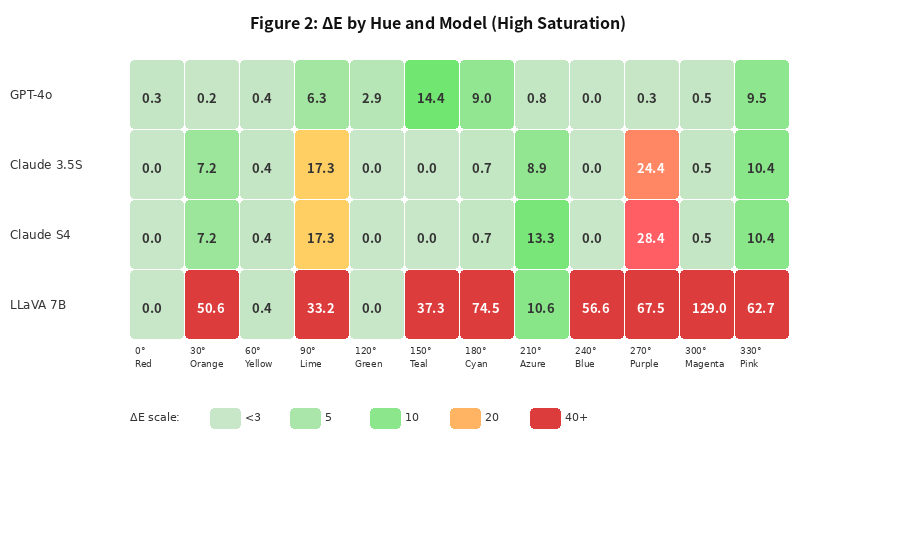
\includegraphics[width=0.85\textwidth]{figures/fig2_hue_heatmap.png}
\caption{CIEDE2000 $\Delta E_{00}$ by hue (columns) and model (rows) at high saturation. Primary colors (0°, 60°, 120°, 240°, 300°) show consistently low error; intermediate hues (90°, 150°, 210°, 270°) show elevated error, particularly for Claude models.}
\label{fig:hue_heatmap}
\end{figure}

All models exhibit strong hue-dependent accuracy patterns (Figure~\ref{fig:hue_heatmap}). At high saturation, primary colors are recognized with near-zero $\Delta E_{00}$, while intermediate hues show significantly higher error:

\begin{itemize}
    \item \textbf{GPT-4o}: Weakest at 150°\ teal ($\Delta E_{00} = 5.88$) and 180°\ cyan ($\Delta E_{00} = 5.43$)
    \item \textbf{Claude 3.5 Sonnet}: Weakest at 270°\ purple ($\Delta E_{00} = 4.24$) and 90°\ lime
    \item \textbf{Claude Sonnet 4}: Similar pattern to 3.5; 270°\ purple ($\Delta E_{00} = 4.24$) is the worst
    \item \textbf{LLaVA 7B}: Uniformly high error across all hues
\end{itemize}

\subsection{Saturation Effects}

Accuracy degrades consistently as saturation decreases. At high saturation ($S=1.0$), commercial models achieve mean $\Delta E_{00} \approx 1$--$2$. At low saturation ($S=0.3$), mean $\Delta E_{00}$ increases to $4$--$6$ for commercial models and exceeds $30$ for LLaVA 7B. This suggests VLMs struggle with desaturated (pastel/muted) colors---precisely the palette range common in modern UI design.

\subsection{Model Version Regression}

Claude Sonnet 4 performs worse than Claude 3.5 Sonnet: higher mean $\Delta E_{00}$ (3.33 vs.\ 3.16) and higher median (3.14 vs.\ 2.95). While the difference is not statistically significant ($p = .727$, $d = -0.05$), the consistent direction of degradation across all metrics suggests a trend worth monitoring. This finding echoes observations in other capability benchmarks where newer model versions do not uniformly improve on all tasks \cite{chen2023}.

\subsection{Cross-Lingual Prompt Comparison (Experiment 2)}

\begin{table}[H]
\centering
\caption{Prompt language effect on color recognition accuracy (high-saturation subset, CIEDE2000).}
\label{tab:prompt_lang}
\begin{tabular}{lrr}
\toprule
\textbf{Model} & \textbf{English} & \textbf{Japanese} \\
\midrule
GPT-4o & 2.33 & 1.71 \\
Claude Sonnet 4 & 1.48 & 1.58 \\
\bottomrule
\end{tabular}
\end{table}

Table~\ref{tab:prompt_lang} shows that prompt language has minimal and inconsistent effect on color recognition accuracy. GPT-4o performs slightly better with Japanese prompts (contrary to expectations for an English-first model), while Claude Sonnet 4 shows negligible difference. This suggests that color perception is primarily a vision capability, not a language-mediated process, and that our main experiment results generalize across languages.

\subsection{UI Component Experiment (Experiment 3)}

\begin{table}[H]
\centering
\caption{Mean $\Delta E_{00}$ by component type (CIEDE2000, 6 colors $\times$ 3 trials).}
\label{tab:ui_components}
\begin{tabular}{lrrr}
\toprule
\textbf{Model} & \textbf{Button} & \textbf{Card} & \textbf{Badge} \\
\midrule
GPT-4o & 1.56 & 1.67 & 1.22 \\
Claude Sonnet 4 & 3.81 & 3.11 & 1.87 \\
\bottomrule
\end{tabular}
\end{table}

Table~\ref{tab:ui_components} shows that VLM color recognition accuracy in realistic UI contexts is comparable to solid-color stimuli, validating the ecological relevance of our main experiment. GPT-4o maintains excellent accuracy (mean $\Delta E_{00} < 2$ across all component types), while Claude Sonnet 4 shows slightly elevated error on buttons ($\Delta E_{00} = 3.81$), possibly due to the visual complexity of text overlays.

\subsection{Accuracy Tier Distribution}

\begin{figure}[H]
\centering
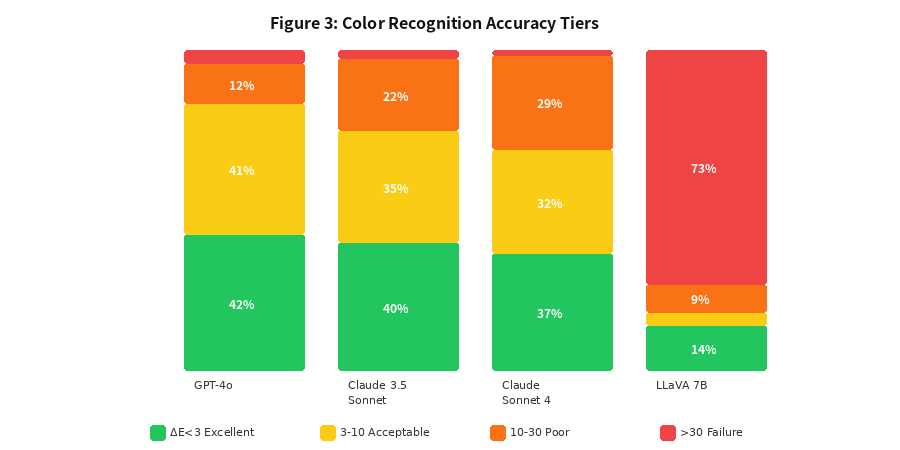
\includegraphics[width=0.7\textwidth]{figures/fig3_accuracy_tiers.png}
\caption{Distribution of responses across accuracy tiers. LLaVA 7B shows 73\% of responses in the ``Failure'' category ($\Delta E_{00} > 10$).}
\label{fig:tiers}
\end{figure}

\subsection{Color Distribution in AI-Generated UIs}

To connect our findings to the AI Slop phenomenon, we analyzed the pixel-level color distribution of seven AI-generated UI sample images (produced using AI design tools for the purpose of this study). Sampling 1,000--2,000 chromatic pixels per image (excluding near-white, near-black, and desaturated regions), we found:

\begin{itemize}
    \item \textbf{95.4\%} of chromatic pixels fall in the 240°\ (blue-purple) hue bin
    \item \textbf{4.6\%} fall in the 210°\ (azure) bin
    \item \textbf{0\%} of sampled AI-generated UI content uses hues outside the 210°--270°\ range
\end{itemize}

While limited in sample size ($n = 7$), this pattern is highly consistent across all analyzed images, suggesting a robust underlying trend rather than a sampling artifact.

This extreme concentration in the blue-purple range directly overlaps with the hue range where VLMs show intermediate accuracy (Section 4.2). Specifically, VLMs demonstrate high accuracy on pure blue (240°, $\Delta E_{00} < 1$) but progressively worse accuracy on nearby intermediate hues (210°\ azure, 270°\ purple). This creates a perverse incentive: AI systems ``see'' pure blue most clearly and may default to it when uncertain, reinforcing the blue-purple convergence.

\section{Discussion}

\subsection{Why Do VLMs Struggle with Intermediate Hues?}

We hypothesize that VLMs' superior performance on primary colors reflects the distribution of color names in training data. Colors like ``red,'' ``blue,'' and ``green'' have unambiguous, high-frequency labels in web text, while intermediate hues like ``teal,'' ``chartreuse,'' or ``mauve'' are rarer and less consistently labeled. This creates a form of \textit{distributional convergence} \cite{bommasani2021} toward well-represented color categories.

This hypothesis is supported by our cross-lingual experiment (Section 4.5): since prompt language has minimal effect on accuracy, the bottleneck appears to be in the vision encoder's mapping of continuous color signals to discrete categories, not in the language model's color vocabulary.

\subsection{The AI Slop Feedback Loop}

Our findings suggest a mechanism by which VLM color biases contribute to the AI Slop phenomenon:

\begin{enumerate}
    \item \textbf{Perception bias}: VLMs perceive primary colors more accurately than intermediate hues (Section 4.2).
    \item \textbf{Color palette narrowing}: When generating UI designs, models default to colors they ``recognize'' well, reducing palette diversity.
    \item \textbf{Training data reinforcement}: As AI-generated UIs (heavily blue-purple) enter training corpora, future models see even more blue-purple, deepening the bias.
    \item \textbf{Empirical evidence}: Our color distribution analysis (Section 4.8) confirms that AI-generated UIs are overwhelmingly concentrated in the 210°--270°\ range.
\end{enumerate}

This constitutes a \textit{feedback loop}: perception bias $\rightarrow$ generation bias $\rightarrow$ training data contamination $\rightarrow$ amplified perception bias.

\subsection{Practical Implications}

For practitioners using AI coding assistants for UI development:
\begin{itemize}
    \item \textbf{Specify colors explicitly}: Use exact HEX codes rather than color names in prompts.
    \item \textbf{Verify intermediate hues}: Pay special attention to teal, lime, and purple in AI-generated designs.
    \item \textbf{Post-generation auditing}: Implement color checking pipelines (e.g., comparing generated CSS values to design tokens).
\end{itemize}

\subsection{Limitations}

\begin{enumerate}
    \item Our main experiment uses solid-color images. While the UI component experiment (Section 4.6) validates ecological relevance for simple components, complex multi-element layouts remain untested.
    \item Three trials per condition provides limited statistical power. Future work should increase trial count for more robust significance testing.
    \item We tested one open-source model (LLaVA 7B). Larger open-source VLMs (e.g., LLaVA 13B, InternVL, Qwen-VL) may show different patterns.
    \item The AI-generated UI samples analyzed in Section 4.8 were produced by the authors. A larger, independently sourced corpus would strengthen the generalizability of the color distribution analysis.
    \item Commercial model versions change over time; our results represent a snapshot as of March 2026.
\end{enumerate}

\section{Conclusion}

We presented a systematic evaluation of color recognition accuracy in four VLMs using CIEDE2000, supplemented by cross-lingual, UI component, and color distribution analyses. Our key findings are:

\begin{enumerate}
    \item Commercial VLMs achieve moderate accuracy (mean $\Delta E_{00}$ 2.51--3.33) but systematically fail on intermediate hues and desaturated colors.
    \item The open-source LLaVA 7B shows substantially lower accuracy ($\Delta E_{00} = 24.63$, $p < 0.001$, $d = -1.75$), suggesting limitations in smaller open-source models that may not generalize to larger variants.
    \item Model updates can degrade color perception (Claude Sonnet 4 vs.\ 3.5).
    \item Prompt language has minimal effect, suggesting color perception is primarily a vision capability.
    \item AI-generated UIs are overwhelmingly concentrated in the blue-purple hue range (95.4\%), overlapping with VLMs' intermediate-accuracy zone.
\end{enumerate}

These findings provide empirical support for a plausible mechanism behind the ``AI Slop'' aesthetic convergence. To the best of our knowledge, this is the first study to quantitatively link VLM color perception biases to the visual homogeneity observed in AI-generated interfaces, offering both theoretical insight and actionable guidance for practitioners building AI-assisted design tools.

\section*{Reproducibility}

All code, stimulus images, raw results, and analysis scripts are available at:\\
\url{https://github.com/kenimo49/ai-blue-color-bias}

\begin{thebibliography}{99}

\bibitem{colorbench2025}
Chen, W., Li, Z., Liu, J., et al.
ColorBench: Can VLMs See and Understand the Colorful World?
\textit{arXiv preprint arXiv:2504.10514}, 2025.

\bibitem{springer2025}
K\"ohler, M., Vetter, S., and Schindler, F.
Advancements and Limitations of LLMs in Replicating Human Color-Word Associations.
\textit{Discover Artificial Intelligence}, 5(1), Springer, 2025.

\bibitem{stanford2025}
Lewis, M. and Lupyan, G.
Blood Is Red, Math Is Blue. Does AI See Colors Like Me and You?
\textit{Stanford Graduate School of Business Working Paper}, 2025.

\bibitem{arxiv2509}
Zaslavsky, N., Maldonado, M., and Culbertson, J.
Culturally Transmitted Color Categories in LLMs Reflect a Learning Bias Toward Efficient Compression.
\textit{arXiv preprint arXiv:2509.08093}, 2025.

\bibitem{rong2024}
Rong, Y., Zhang, L., and Wang, H.
Analyzing the Color Availability of AI-Generated Posters Based on K-Means Clustering.
\textit{Color Research \& Application}, 49(3), Wiley, 2024.

\bibitem{macquarie2025}
Macquarie Dictionary.
AI Slop Named 2025 Word of the Year.
\textit{Macquarie Dictionary Blog}, December 2025.
Merriam-Webster.
AI Slop Named 2025 Word of the Year.
\textit{Merriam-Webster Press Release}, December 2025.

\bibitem{ciede2000}
Sharma, G., Wu, W., and Dalal, E.N.
The CIEDE2000 Color-Difference Formula: Implementation Notes, Supplementary Test Data, and Mathematical Observations.
\textit{Color Research \& Application}, 30(1):21--30, 2005.

\bibitem{bommasani2021}
Bommasani, R., Hudson, D.A., Adeli, E., et al.
On the Opportunities and Risks of Foundation Models.
\textit{arXiv preprint arXiv:2108.07258}, 2021.

\bibitem{chen2023}
Chen, L., Zaharia, M., and Zou, J.
How Is ChatGPT's Behavior Changing over Time?
\textit{arXiv preprint arXiv:2307.09009}, 2023.

\end{thebibliography}

\end{document}
